%%%%%%%%%%%%%%%%%%%%%%%%%%%%%%%%%%%%%%%%%
% Large Colored Title Article
% LaTeX Template
% Version 1.1 (25/11/12)
%
% This template has been downloaded from:
% http://www.LaTeXTemplates.com
%
% Original author:
% Frits Wenneker (http://www.howtotex.com)
%
% License:
% CC BY-NC-SA 3.0 (http://creativecommons.org/licenses/by-nc-sa/3.0/)
%
%%%%%%%%%%%%%%%%%%%%%%%%%%%%%%%%%%%%%%%%%

%----------------------------------------------------------------------------------------
%	PACKAGES AND OTHER DOCUMENT CONFIGURATIONS
%----------------------------------------------------------------------------------------

\documentclass[DIV=calc, paper=a4, fontsize=12pt, twocolumn]{scrartcl}	 % A4 paper and 11pt font size


\usepackage{fix-cm}	 % Custom font sizes - used for the initial letter in the document
\usepackage{hyperref}
\hypersetup{colorlinks=true}

\usepackage{lipsum} % Used for inserting dummy 'Lorem ipsum' text into the template		
\usepackage[english]{babel} % English language/hyphenation		
\usepackage[protrusion=true,expansion=true]{microtype} % Better typography		
\usepackage{amsmath,amsfonts,amsthm} % Math packages		
\usepackage[svgnames]{xcolor} % Enabling colors by their 'svgnames'		
\usepackage[hang, small,labelfont=bf,up,textfont=it,up]{caption} % Custom captions under/above floats in tables or figures		
\usepackage{booktabs} % Horizontal rules in tables
\usepackage{graphicx}
\usepackage{afterpage}

\usepackage{fancyhdr} % Needed to define custom headers/footers
\pagestyle{fancy} % Enables the custom headers/footers
\usepackage{lastpage} % Used to determine the number of pages in the document (for "Page X of Total")

% Headers - all currently empty
\lhead{}
\chead{}
\rhead{}

% Footers
\lfoot{}
\cfoot{}
\rfoot{\footnotesize Page \thepage\ of \pageref{LastPage}} % "Page 1 of 2"
\usepackage{sectsty} % Enables custom section titles		
\renewcommand{\headrulewidth}{0.0pt} % No header rule
\renewcommand{\footrulewidth}{0.4pt} % Thin footer rule

\usepackage{lettrine} % Package to accentuate the first letter of the text
\newcommand{\initial}[1]{ % Defines the command and style for the first letter
\lettrine[lines=3,lhang=0.3,nindent=0em]{
\color{DarkGoldenrod}
{\textsf{#1}}}{}}

%----------------------------------------------------------------------------------------
%	TITLE SECTION
%----------------------------------------------------------------------------------------

\usepackage{titling} % Allows custom title configuration

\newcommand{\HorRule}{\color{DarkGoldenrod} \rule{\linewidth}{1pt}} % Defines the gold horizontal rule around the title

\pretitle{\vspace{-30pt} \begin{flushleft} \HorRule \fontsize{50}{50} \usefont{OT1}{phv}{b}{n} \color{DarkRed} \selectfont} % Horizontal rule before the title

\title{Applications of Computer Vision in Textiles} % Your article title

\posttitle{\par\end{flushleft}\vskip 0.5em} % Whitespace under the title

\preauthor{\begin{flushleft}\large \lineskip 0.5em \usefont{OT1}{phv}{b}{sl} \color{DarkRed}} % Author font configuration

\author{Dr. Samrat Mukhopadhyay\newline Robin Malhotra(2012TT10951), Rahul Sharma(2012TT10946) } % Your name

\postauthor{\footnotesize \usefont{OT1}{phv}{m}{sl} \color{Black} % Configuration for the institution name
Indian Institute of Technology, Delhi % Your institution

\par\end{flushleft}\HorRule} % Horizontal rule after the title

\date{February 27,2015} % Add a date here if you would like one to appear underneath the title block

%----------------------------------------------------------------------------------------

\begin{document}

\maketitle % Print the title

\thispagestyle{fancy} % Enabling the custom headers/footers for the first page 

%----------------------------------------------------------------------------------------
%	ABSTRACT
%----------------------------------------------------------------------------------------

% The first character should be within \initial{}
\initial{W}\textbf{ith the advent of computers and automation practices, Computer Vision has found use in various applications- from looking for cracks in building foundations to observing plant growth in greenhouses. In this Mini Project (under the able guidance of Prof. Samrat Mukhopadhyay), we are going to explore the possibilities of using this technology for Quality asssurance in the textile industry. }

%----------------------------------------------------------------------------------------
%	ARTICLE CONTENTS
%----------------------------------------------------------------------------------------
\section{Work done till now}
In the past one month, we have successfully completed the hardware project. We have procured all parts required- a raspberry pi( credit card-sized single-board computer), associated CSI camera and the requisite software tools(python3.4 and openCV, to be precise) for the project. We have assembled a cardboard-and-glue prototype for capturing images and testing. We have also familiarised ourselves with the integration of the raspberry pi camera. We have also completed a literature review of a few research papers from sources like IEEE, Hong Kong University etc. In the following sections we shall discuss the mathematical logic and algorithms that we plan to incorporate in our software application as well as the challenges we shall face.

\section{Current Industry State}

While the current industry has attempted to use Computer Vision and Image Processing for Quality Assurance, attempts have often been expensive and cumbersome. Take the example of  \href{http://www.avt-inc.com/?catid=\%7B757EF709-E4DF-4C16-A2E7-5F7866D891AC\%7D}{AVT Inc, Israel} that sells high quality instruments that use spectral imaging techniques to look for defects in fabrics. While these techniques may be useful and necessary in fabrics for aeronautical and structural purposes, this appears to be plain and simple overkill for garment fabrics. Also, research in this field has more or less remained stagnant after 2006, leaving the algorithms that run these processes fairly inefficient.

\section{Algorithms and logic}

We have reviewed several findings and research papers(our internet history from yesterday should be a testament to that). Here we will discuss the standard methods used by various researchers across the world.
\begin{itemize}

\item Our first challenge is to count the ends per inch(epi) and picks per inch(ppi). The algorithm behind this, ironically was not found in research labs, but on a code challange!
\begin{enumerate}	
\item Refer to the rice grain challenge on Stackexchange. \href{http://codegolf.stackexchange.com/questions/40831/counting-grains-of-rice}{Link}
\item Several methods were proposed by the participants, involving adaptive thresholds, deep learning, watershed algorithms and other mathematics that doesn't make sense to me.
\item Some surprisingly simple algorithms worked deceptively well for this problem. 
\item Idea : scan the image, one row at a time. For each line, count the number rice grains encountered (by checking if pixel turns black to white or the opposite). If number of grains for the line increase (compared to previous line), it means we encountered a new grain. If that number decrease, it means we passed over a grain. In this case, add +1 to the total result.
\end{enumerate}
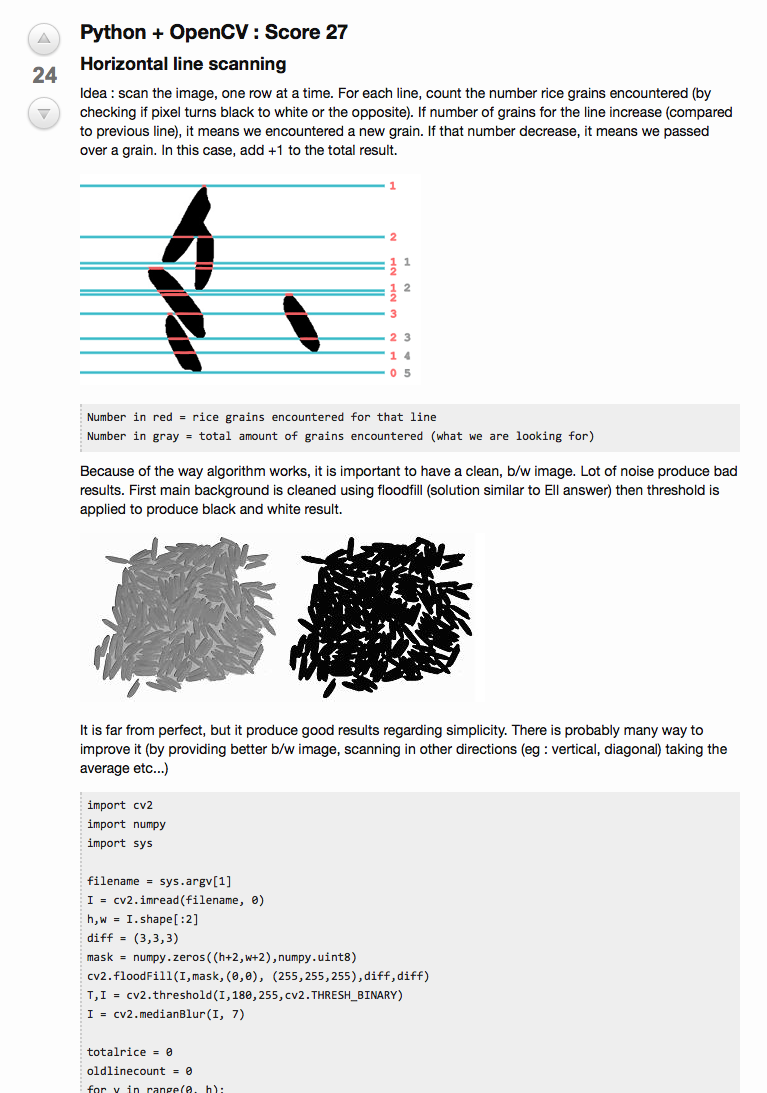
\includegraphics[width=0.4\textwidth]{/Users/robinmalhotra2/Developer/OpenCV/image4.png}


\item One of the most popular techniques is edge detection using Gabor filters. Its impulse response is defined by a sinusoidal wave (a plane wave for 2D Gabor filters) multiplied by a Gaussian function. A set of Gabor filters with different frequencies and orientations may be helpful for extracting useful features from an image. Gabor filters have been widely used in pattern analysis applications. In the research paper by \href{http://hub.hku.hk/bitstream/10722/46561/1/131190.pdf}{HKU}, this technique is used extensively for plain, twill and denim fabrics.  
\textbf{Filter selection and detection Algorithm:}
\begin{enumerate}
\item $g_c(x,y)=e^{-\frac{1}{2} \big[ \big(\frac{ x^{'}}{\sigma_x} \big)^2 +  \big(\frac{ y^{'}}{\lambda \sigma_x} \big)^2 \big]} \cos \big[2\pi \mu_0 x^{'}\big]$
where   $x^{'}$ and  $y^{'}$ are the rotated transformed values of the x and y coordinates.$ \mu_0$ is the frequency of a sinusoidal wave along the x axis and $\lambda$ is the ratio between the variances in the y and x directions.
\item $E=\sum_{x,y}\big[ IM(x,y)-w^{i}g_{e}^{i}(x,y) \big]^{2}$
where g is the gabor function in x,y 
 \item By minimising the above function, we create an optimal solution from a set of 7 real filters(by changing various parameters). Generally the size of defects is greater than a yarn, the filtering results with finer resolutions than a yarn contribute very little for segmenting defects.
\item $O_f=\sum_{i=1}^{J} a^i f^i \big( f^i= IM*g_e^i ; a^i=\alpha^i / \sum_{k=1}^{J} \alpha^k \big)$
Note that the image data here is the fourier convolution.
\item Finally,the final binary segmentation result of a fabric is obtained by thresholding output from  the median filtering step.

\end{enumerate}

\item \textbf{Defect detection using bi-level thresholding:}Another method for defect detection is bilevel thresholding. This involves scanning across the width  of the grayscale image.
\begin{enumerate}
\item We will first define a threshold value for intensity that will be used to contrast the defect/yarns for counting(whatever may be the case).  
\item A histogram is plotted with greyscale intensity vs pixels to produce 2 sets of pixels: $G_1$ consisting of pixels with grey level $T\geq T_1$ and $G_2$ with $T\geq T_2$. We will then find the average value $\mu_1$ and $\mu_2$ for these 2 regions.
\item Then the value of T can be computed as $T=\frac{1}{2} \big( \mu_1 + \mu_2 \big)$  
\item We can repeat this algorithm until our difference in successive iterations is lower than a bound $T_0$
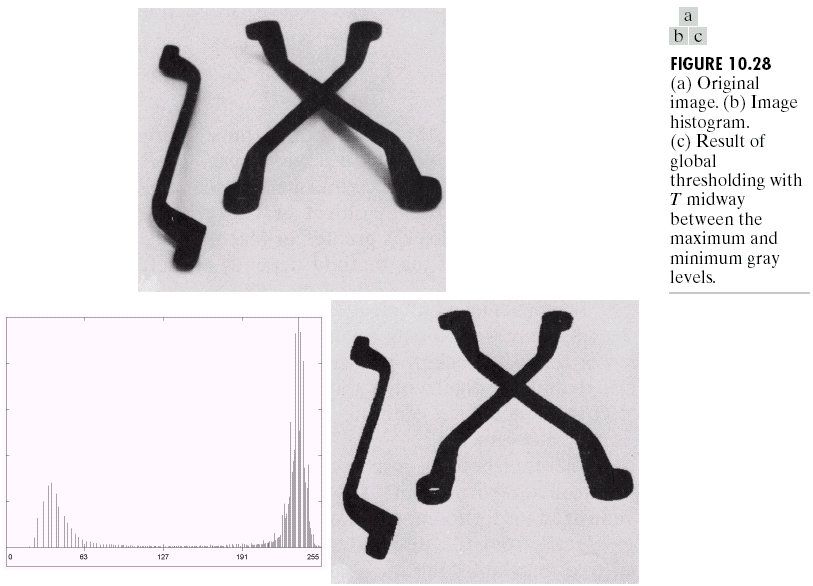
\includegraphics[width=0.4\textwidth]{/Users/robinmalhotra2/Developer/OpenCV/image3.png}

\item Note that this was the probable idea used by our predecessors in the TTP200 course. 
\item A few factors working for us in this case is that we can accurately control the lighting and aperture etc of the camera, which should give us distinct peaks/valleys in the histogram.
\item This method, however, will not work well with patterned fabrics.
\end{enumerate}

\item The last method is Fractal Dimensions. This basically tries to detect an irregular geometric object with an infinite nesting of structure at all scales. The localization accuracy of these detected defects is very poor and have high false alarm. 

\begin{enumerate}
\item An important (defining) property of a fractal is self-similarity, which refers to an infinite nesting of structure on all scales. 
\item Strict self- similarity refers to a characteristic of a form exhibited when a substructure resembles a superstructure in the same form.
\item A great way to explain fractals is \href{http://www.shodor.org/master/fractal/software/Snowflake.html#HELPLIST}{here}
\item The Japanese have extensively researched the possibility of using fractals to create intricate \href{http://www.shodor.org/master/fractal/software/Snowflake.html#HELPLIST}{designs}
\end{enumerate}
For more information, refer \href{http://www.vanderbilt.edu/AnS/psychology/cogsci/chaos/workshop/Fractals.html}{here}
\end{itemize}

\section{Plan for the future}
Our plan for the rest of the semester involves implementing these algorithms in python till a usable product is achieved. We are also planning to improve our prototype with a macro lens system, as well as a mechanism for adjusting focus.
\clearpage


\includegraphics[width=\textwidth]{/Users/robinmalhotra2/Developer/OpenCV/Gabor-ocr.pdf}
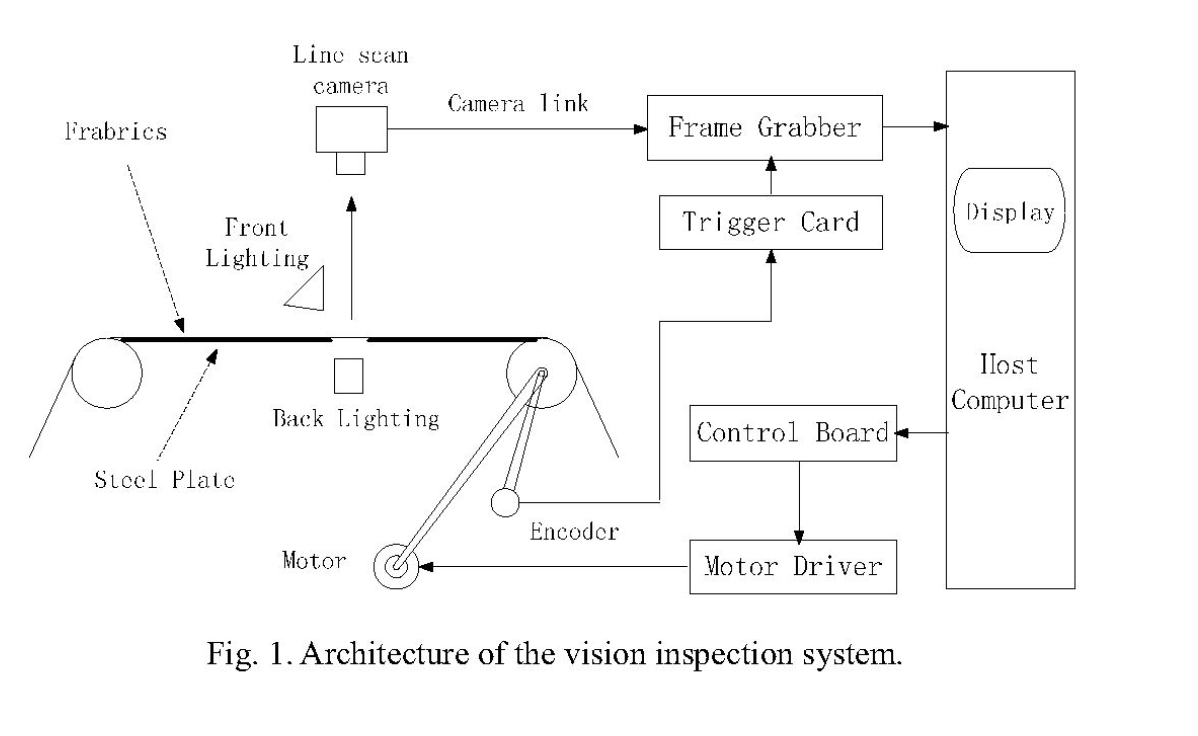
\includegraphics[width=\textwidth]{/Users/robinmalhotra2/Developer/OpenCV/Plan}
\newpage
\clearpage
\begin{center}
 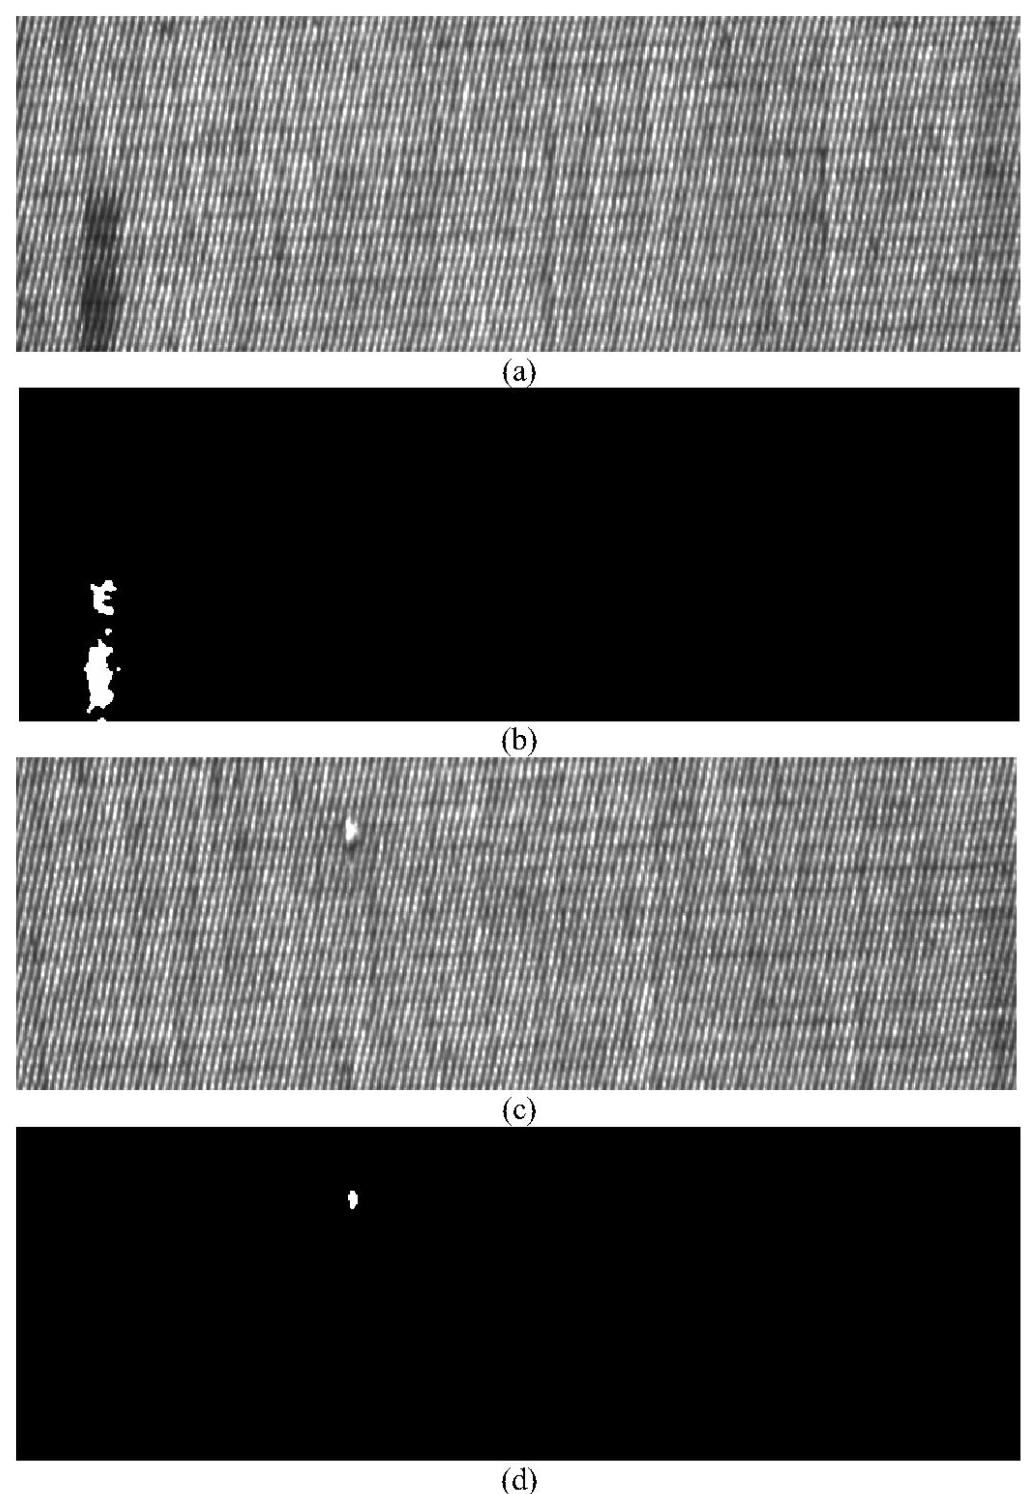
\includegraphics[width=0.9\textwidth]{/Users/robinmalhotra2/Developer/OpenCV/flowChart.png}
System Performance
\end{center}


\clearpage
\newpage
%----------------------------------------------------------------------------------------
%	REFERENCE LIST
%----------------------------------------------------------------------------------------

\begin{thebibliography}{99} % Bibliography - this is intentionally simple in this template

\bibitem[Mak, K.L.; Peng, P.; Lau, H.Y.K]{doi: 10.1109/ICIT.2005.1600684}
\newblock AA real-time computer vision system for detecting defects in textile fabrics
\newblock {\em IEEE International Conference}
 
\bibitem[www.csie.ntpu.edu.tw]{doi: 10.1109/ICIT.2005.1600684}
\newblock $www.csie.ntpu.edu.tw/~dalton/course/Computer_Vision/.../Chapter_4.ppt$ 




\end{thebibliography}

%----------------------------------------------------------------------------------------

\end{document}